\subsubsection{Bayesian reweighting analysis}
\label{sec:projections:rw}

To quantify the impact of future lattice-QCD calculations on global fits 
in each of the three scenarios in Table~\ref{tab:scenarios},
we use a procedure based on Bayesian reweighting analysis.
%
We briefly describe this procedure here, and refer 
to~\cite{Ball:2011gg,Ball:2010gb} for additional details.

\begin{itemize}

\item We first generate pseudo-data for the lattice-QCD calculations
of $\la x\ra_{u^+}$, $\la x\ra_{d^+}$, $\la x\ra_{s^+}$,
$\la x\ra_{g}$, and $\la x\ra_{u^+-d^+}$ (for the unpolarized case), and
$\la 1\ra_{\Delta u^+}$, $\la 1\ra_{\Delta d^+}$,
$\la 1\ra_{\Delta s^+}$, $\la x\ra_{\Delta u^--\Delta d^-}$, and
$\la 1\ra_{\Delta u^+ - \Delta d^+}$ (for the polarized case).
%
We denote generically these moments by $\mathcal{F}_i$.
  
\item We construct the associated pseudo-data, denoted by 
$\mathcal{F}_i^\text{(exp)}$, by taking the central values from
the corresponding NNPDF fits, NNPDF3.1 NNLO for the unpolarized case and 
NNPDFpol1.1 NLO for the polarized case.
%
That is, we {\it assume} for simplicity that the central value
of such future lattice calculations would coincide with the current ones
from the global fit.\footnote{ The exercise can be repeated
 with the actual lattice-QCD central values. However, this 
 requires some choices, such as to how to impose 
 the momentum sum rule.
 This is beyond the scope of the present studies.}
%
As discussed in Sec.~\ref{sec:unpPDFs}, this corresponds to computing
the mean over the Monte Carlo replica sample,
\be
\label{eq:pseudodatadef}
\mathcal{F}_i^\text{(exp)} \equiv \frac{1}{N_\text{rep}}\sum_{k=1}^{N_\text{rep}}
\mathcal{F}_i^{(k)} \, , \quad i=1,\ldots,N_\text{mom} \, ,
\ee
where $N_\text{mom}$ is the number of PDF moments that will be included
in the reweighting; here $N_\text{mom}=5$ both for the unpolarized and 
polarized cases.
%
To be consistent with the calculations in Sec.~\ref{sec:benchmarking},
the central values of the pseudo-data, Eq.~\eqref{eq:pseudodatadef},
are also evaluated at $Q^2=4\text{ GeV}^2$ 
(see Tables~\ref{tab:unpPDFmoms} and \ref{tab:polPDFmoms}).

\item The uncertainty in the pseudo-data, denoted by 
$\delta\mathcal{F}_i^\text{(exp)} $, is taken to be the value indicated in
Table~\ref{tab:scenarios} for each of the three scenarios.
%
Thus, the absolute uncertainty on the $i$-th moment
is given by 
$\delta\mathcal{F}_i^\text{(exp)}=\delta_L^{(i)}\mathcal{F}_i^\text{(exp)} $.

\item Using the pseudo-data (central values and total uncertainties)
as defined above, we compute the Bayesian weights $\omega_k$.
%
These weights quantify the agreement between each $k$-th replica in 
the input PDF set and the corresponding lattice pseudo-data.
%
We compute the $\chi^2$ for each replica $k$ as
\be
\chi^{2(k)}= \sum_{i=1}^{N_\text{mom}} \frac{\lp
\mathcal{F}_i^{(k)} -\mathcal{F}_i^\text{(exp)} \rp^2}{
\lp \delta\mathcal{F}_i^\text{(exp)}\rp^2} \, , \quad k=1,\ldots,N_\text{rep} \, ,
\ee
assuming that there are no correlations between different $N_\text{mom}$ moments.
%
This assumption in general might not be a good approximation, since most 
lattice-QCD systematic errors are correlated among different moments, 
and can be avoided, provided the full breakdown of systematic errors 
for each quantity is available.
  
Once the values of the $\chi^2$ have been evaluated,
we compute the corresponding weights for each replica.
%
The relation between the weights $w_k$  and the values of
the $\chi^{2(k)}$ of each replica is~\cite{Ball:2011gg,Ball:2010gb}
\be
\omega_k =\frac{\lp \chi^{2(k)} \rp^{(N_\text{mom}-1)/2}\exp(-\chi^{2(k)}/2)}{
\sum_{k=1}^{N_\text{rep}} \lc \lp \chi^{2(k)} \rp^{(N_\text{mom}-1)/2}\exp(-\chi^{2(k)}/2)\rc} \, ,
\ee
where the denominator ensures that the weight admits
a probabilistic interpretation, that is, $\sum_k w_k=1$.
%
These weights represent a measure of the agreement of the individual replicas 
with the new pseudo-data.
%
For instance, replicas which have associated values of the moments far from 
the pseudo-data (within uncertainties) will have a large $\chi^2$ and a 
very small weight, being thus effectively discarded.

\item These weights are used to recompute the PDFs, their moments,
and generic cross-sections.
%
This procedure emulates the
impact of adding lattice-QCD pseudo-data to a complete PDF fit.
%
For instance, after reweighting, the mean value of
the PDF moments is
\be
\label{eq:pseudodatadef1}
\mathcal{F}_i^\text{(rw)} = \sum_{k=1}^{N_\text{rep}}\omega_k
\mathcal{F}_i^{(k)} \, , \quad i=1,\ldots,N_\text{mom} \, ,
\ee
with a similar relation for the associated uncertainties.
\end{itemize}

One limitation of the reweighting procedure is that it is maximally 
reliable if the effective number of replicas $N_\text{eff}$ that survive the 
reweighting procedure (which is a measure of the amount
of information left) is not too small.
%
This effective number of replicas is quantified in terms of the Shannon 
entropy~\cite{Ball:2011gg,Ball:2010gb}
\be
\label{eq:effnrep}
N_\text{eff}\equiv \exp\lc \frac{1}{N_\text{rep}}\sum_{k=1}^{N_\text{rep}}\omega_k
\log \lp N_\text{rep}/\omega_k\rp\rc \, .
\ee
%
Finding $N_\text{eff}\ll N_\text{rep}$ means that the pseudo-data
have a large impact on the fit, potentially leading to a large
reduction of the PDF uncertainties.
%
If either the effective number of replicas becomes too small 
(say $N_\text{eff}\lsim 25$), or the relative fraction is small 
(say, $N_\text{eff}/N_\text{rep}\lsim 0.10$), then the results become unreliable, 
since they are affected by large statistical fluctuations.

Therefore, before considering the effects
of the lattice-QCD pseudo-data at the PDF
level, we need to ensure that the
three scenarios defined
in Table~\ref{tab:scenarios} still lead
to values of $N_\text{eff}$ large enough for
the reweighting procedure to be reliable.
%
In Table~\ref{tab:neff} we indicate the effective number of replicas
$N_\text{eff}$, Eq.~\eqref{eq:effnrep}, remaining when the pseudo-data
are included in the global
fit according to the scenarios in Table~\ref{tab:scenarios}.
%
For completeness, we also quote the original number
of replicas $N_\text{rep}$ for the prior
PDF sets, NNPDF3.1 and NNPDFpol1.1, respectively.
%
As we can see, there is a marked decrease of $N_\text{rep}$
for the three scenarios, indicating that adding the
PDF moments leads to non-trivial constraints on the global fit.
%
For instance, in the most optimistic scenario, Scenario~C, the effective 
number of replicas is around two (five) times smaller than the starting 
number of replicas in the unpolarized (polarized) case.

%-------------------------------------------------------------------------------
\begin{table}[!t]
\centering
\footnotesize
\renewcommand{\arraystretch}{1.3} 
\begin{tabular}{lcc}
\toprule
&  NNPDF3.1  &  NNPDFpol1.1 \\
\midrule
$N_\text{rep}$ original   &   1000 &  100   \\
$N_\text{eff}$ Scenario A    &   740  &  72   \\
$N_\text{eff}$ Scenario B    &   750   &   59  \\
$N_\text{eff}$ Scenario C   &   510  &   20  \\
\bottomrule
\end{tabular}
\caption{\small The effective number of replicas
$N_\text{eff}$, Eq.~\eqref{eq:effnrep}, remaining after pseudo-data
on the PDF moments are included in the global
fit according to the scenarios outlined
in Table~\ref{tab:scenarios}.
%
For completeness, we also indicate the original number
of replicas $N_\text{rep}$ for the prior
PDF sets, NNPDF3.1 and NNPDFpol1.1.
\label{tab:neff}}
\end{table}
%-------------------------------------------------------------------------------

\paragraph{Impact on unpolarized global fits.}
\label{subsec:upolfits}
%
We now discuss the results of applying the reweighting procedure to NNPDF3.1.
%
In Table~\ref{tab:unpolmomentsrw} we summarize
the values of the unpolarized PDF moments
used as pseudo-data $\mathcal{F}_i^{(\rm exp)}$,
and the corresponding results
after the reweighting has been performed, for the
three scenarios summarized 
in Table~\ref{tab:scenarios};
PDF uncertainties correspond to 68\%-CL intervals.
%
We recall that, as explained above, the three scenarios exhibit
uncertainties $\delta_L^{(i)}$ for the lattice-QCD pseudo-data rather smaller
than those of current state-of-the-art
calculations (see Table~\ref{tab:BMunp}).

%-------------------------------------------------------------------------------
\begin{table}[!t]
\centering
\footnotesize
\renewcommand{\arraystretch}{1.4} 
\begin{tabular}{lcccc}
\toprule 
&  Original  & Scenario A  &  Scenario B  &  Scenario C  \\
\midrule
$\la x\ra_{u^+}$     
& $0.348 \pm 0.005$ 
& $0.349 \pm 0.004$ 
& $0.349 \pm 0.004$ 
& $0.349 \pm 0.003$ \\
$\la x\ra_{d^+}$     
& $0.196 \pm 0.004$     
& $0.196 \pm 0.004$       
& $0.196 \pm 0.003$ 
& $0.196 \pm 0.002$ \\
$\la x\ra_{s^+}$     
& $0.0393 \pm 0.0036$   
& $0.0389 \pm 0.0030$   
& $0.0389 \pm 0.0024$   
& $0.0389 \pm 0.0014$  \\
$\la x\ra_{g}$       
& $0.4097 \pm 0.0042$    
& $0.4097 \pm 0.0043$    
& $0.4097 \pm 0.0040$ 
& $0.4097 \pm 0.0029$  \\
$\la x\ra_{u^+-d^+}$  
& $0.1522 \pm 0.0033$   
& $0.1521 \pm 0.0037$   
& $0.1521 \pm 0.0035$ 
& $0.1521 \pm 0.0029$ \\
\bottomrule
\end{tabular}
\caption{\small Values of the unpolarized PDF moments
  used as pseudo-data, as well as the corresponding results
  after the reweighting has been performed, for the
  three scenarios summarized 
  in Table~\ref{tab:scenarios}.
  %
  The PDF uncertainties quoted correspond in all cases to 68\% CL intervals.
\label{tab:unpolmomentsrw}}
\end{table}
%-------------------------------------------------------------------------------

From Table~\ref{tab:unpolmomentsrw} we see that a significant
reduction in the uncertainties in the unpolarized PDF moments is challenging 
to achieve unless we assume the most aggressive scenarios.
%
For instance, in Scenario~C, which is about the best precision that
can be achieved from lattice-QCD in the near future, the PDF uncertainties 
of the first moments (that is, the momentum fractions) for $u^+,d^+,s^+$ and 
$g$ decrease by around 30\%--60\%.
%
The most marked decrease is for the strange momentum fraction, since this is 
affected by the largest PDF error in the prior fit.
%
In contrast, the nonsinglet combination $\la x\ra_{u^+-d^+}$ is essentially
unchanged in all three scenarios.
%
Note that, in Table~\ref{tab:unpolmomentsrw}, the central values of the PDF 
moments are stable, since we assume that the central values of the 
pseudo-data correspond to those of the input PDFs. 
%
In a realistic situation, this is not necessarily the case and 
central values of the PDFs could also vary.

%-------------------------------------------------------------------------------
\begin{figure}[!t]
\centering
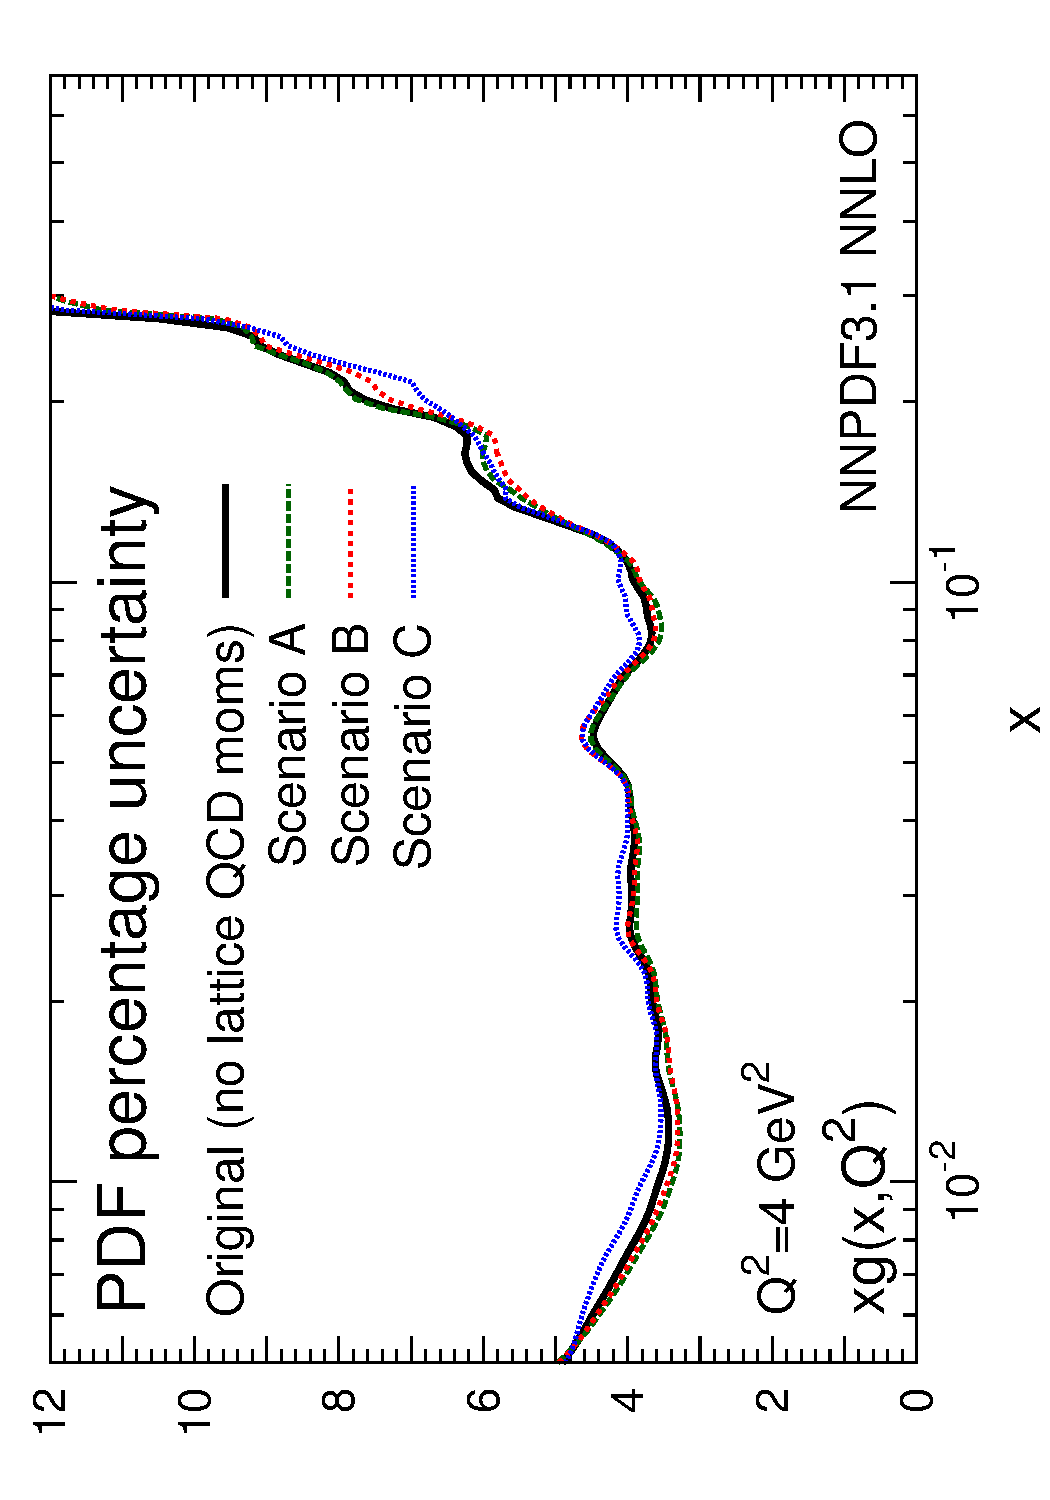
\includegraphics[angle=270,scale=0.35]{plots/UNPg}
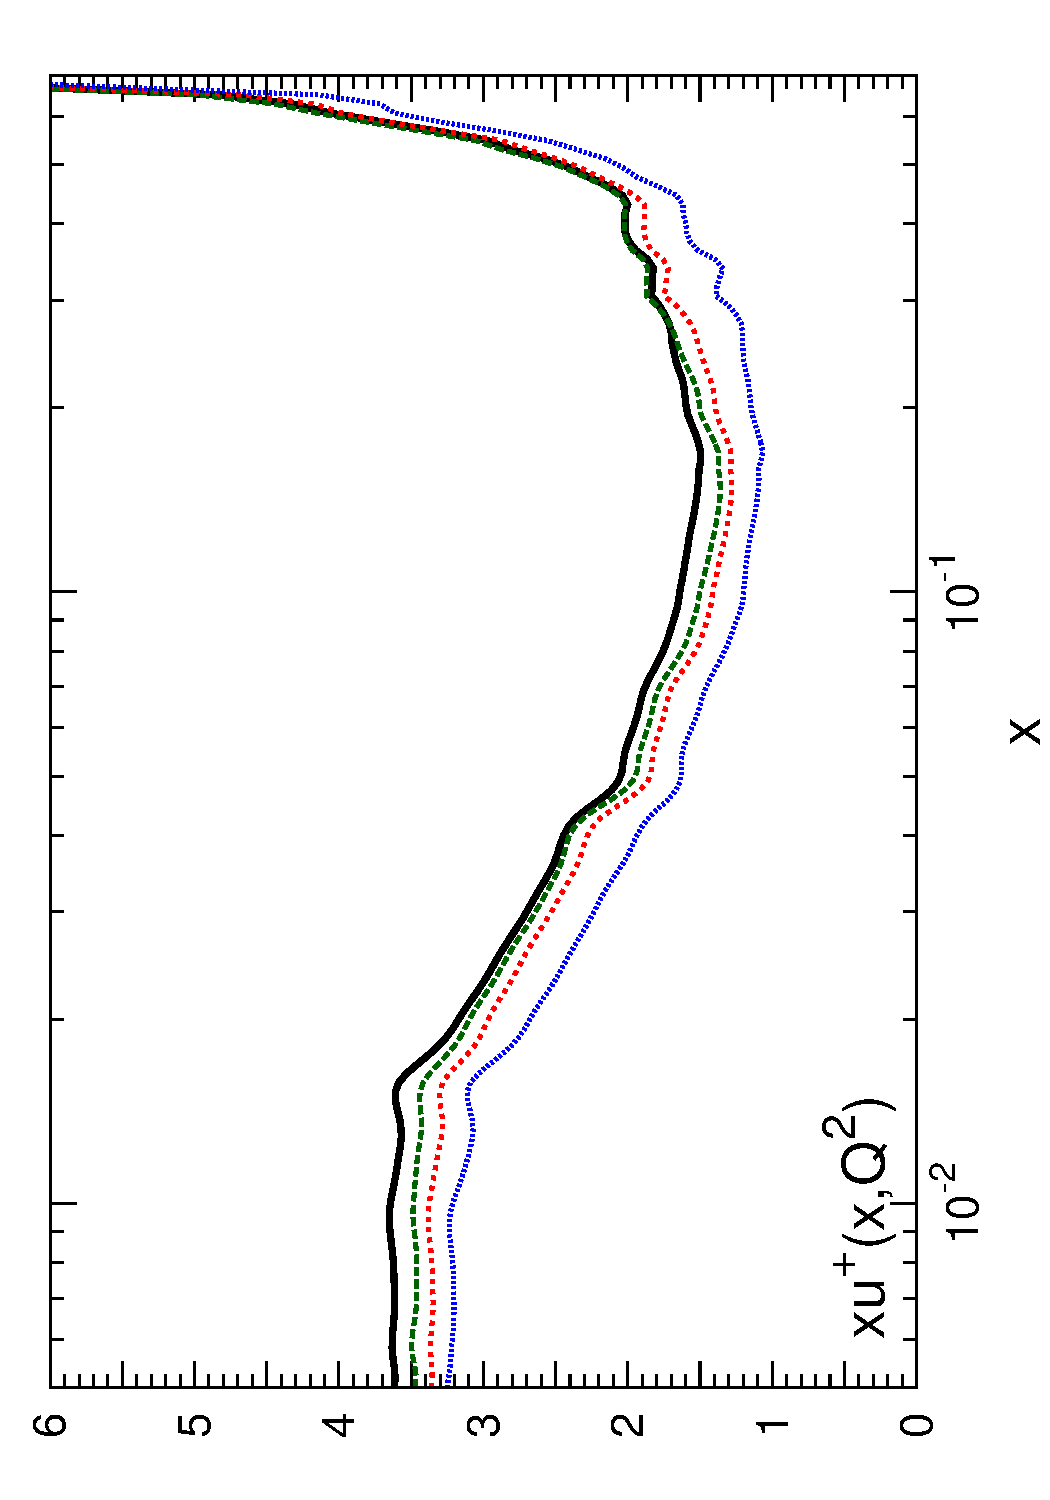
\includegraphics[angle=270,scale=0.35]{plots/UNPu}\\
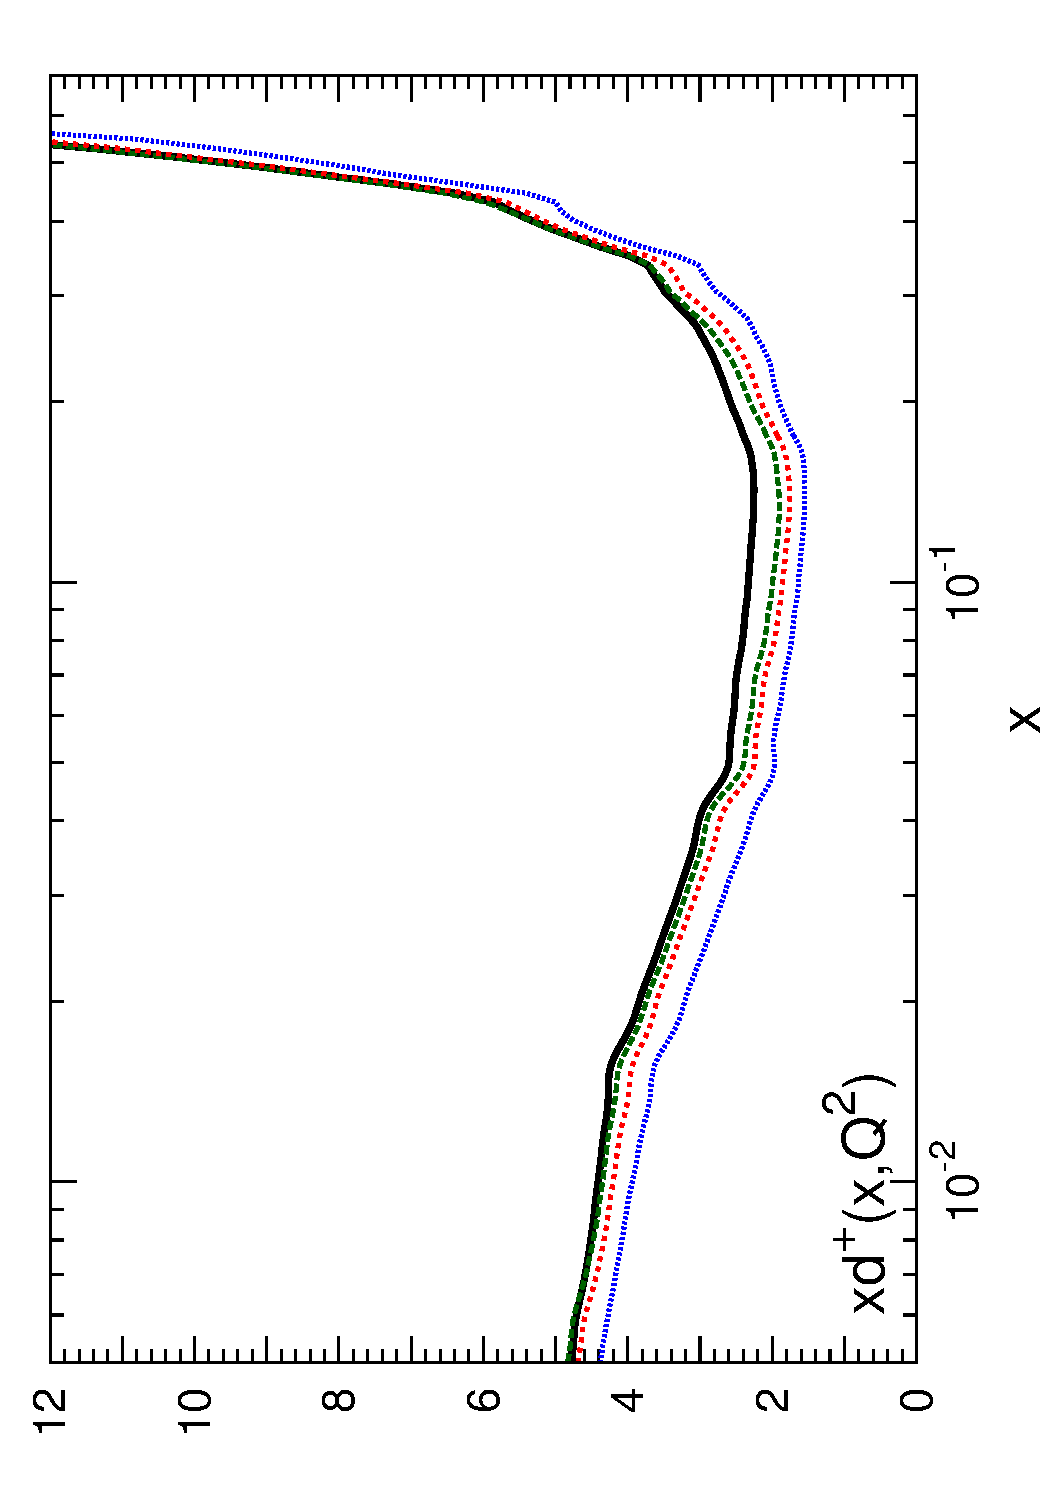
\includegraphics[angle=270,scale=0.35]{plots/UNPd}
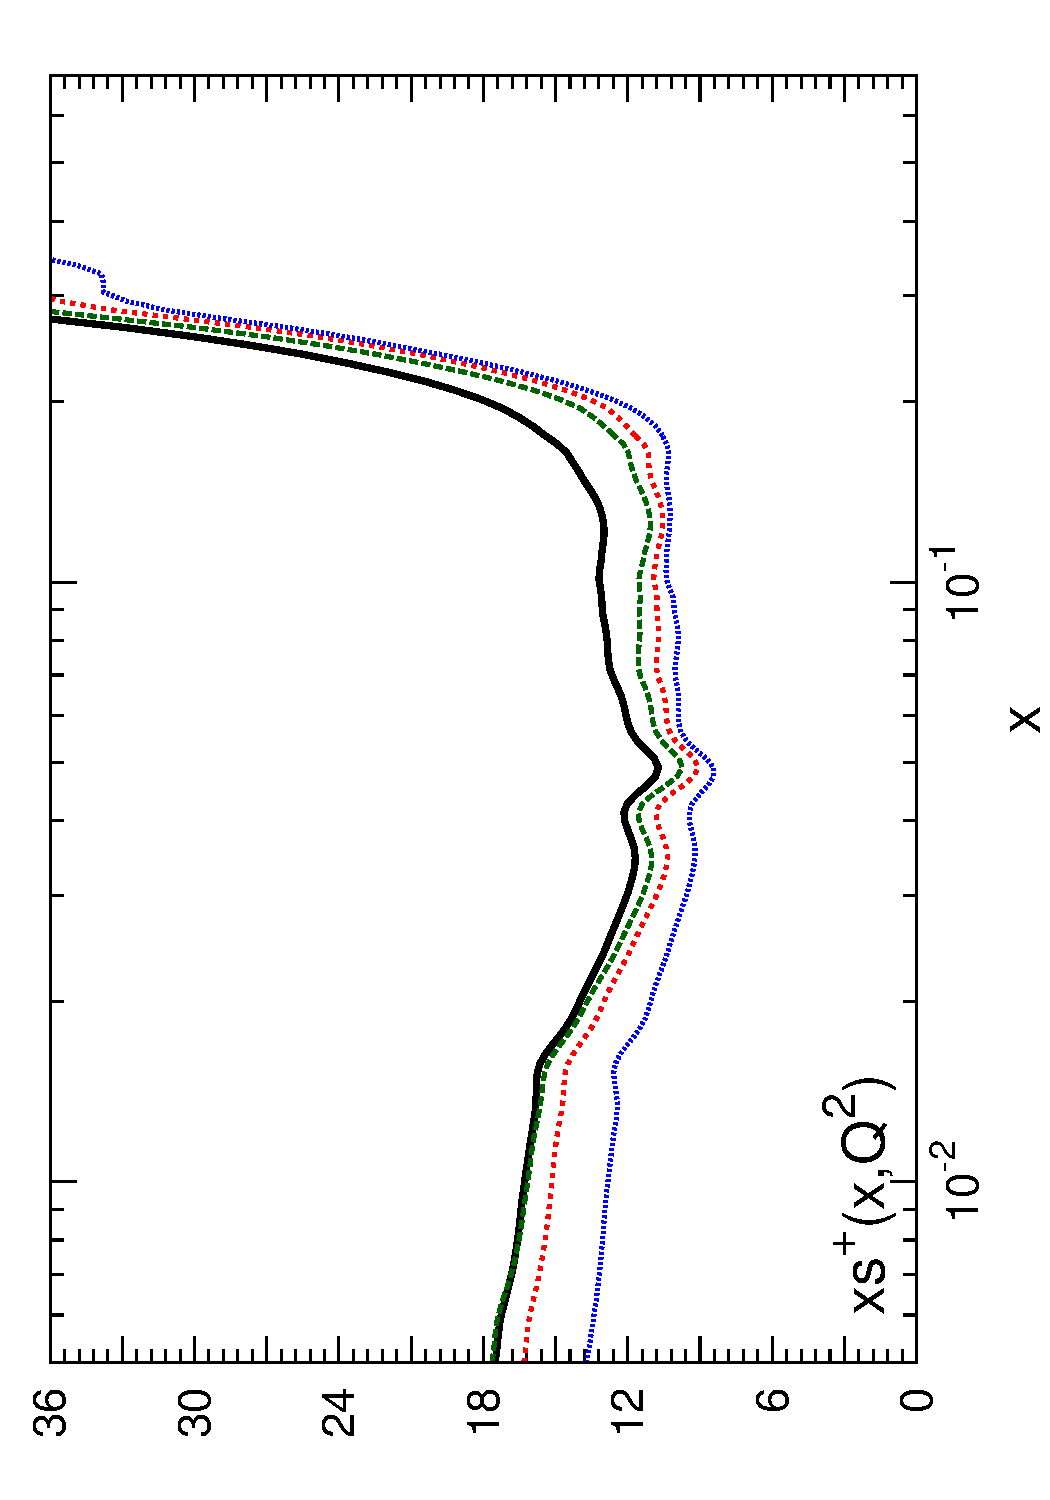
\includegraphics[angle=270,scale=0.35]{plots/UNPs}\\
\caption{\small The percentage PDF uncertainty in NNPDF3.1  
  for the gluon and the $u^+$, $d^+$ and $s^+$ quark PDFs at
  $Q^2=4\text{ GeV}^2$,
  compared to the results of including lattice-QCD pseudo-data for
  moments of PDFs in the fit, according to the three
  scenarios in Table~\ref{tab:scenarios}.
  %
  See text for details.
}    
\label{fig:impactUnpol}
\end{figure}
%----------------------------------------------------------

Further evidence that reducing uncertainties in unpolarized PDFs will be 
challenging is shown in Fig.~\ref{fig:impactUnpol}, which displays the 
percentage PDF uncertainties in NNPDF3.1 for the gluon and the
$u^+$, $d^+$ and $s^+$ quark PDFs at $Q^2=4\text{ GeV}^2$, compared to the 
corresponding results including lattice-QCD pseudo-data.
%
In the case of the $u^+,d^+$ and $s^+$, we observe a slight reduction
of the PDF uncertainties, which is more marked as we move
from Scenarios~A to C.
%
For instance, in the latter case the percentage PDF
uncertainty on $u^+$ ($d^+$ and $s^+$) at $x\simeq 0.1$
decreases from 1.8\% to 1.2\% (from 2.2\% to 1.7\% and from 13\% to 10\%, 
respectively).
%
The PDF uncertainties of the gluon PDF, however,
are essentially unchanged even in the most optimistic scenario.

We also observe the trend that the reduction of the uncertainty 
of the PDF moments (see Table~\ref{tab:unpolmomentsrw})
is more significant than the PDF uncertainty as a function of $x$  
(Fig.~\ref{fig:impactUnpol}).
%
We will see that this pattern also persists for the polarized PDF case.
%
As the PDF moments integrate across all $x$ values (with emphasis on 
smaller $x$ values), this suggests that there are correlations which could be 
driving this result.
%
In particular we note that in Scenario~C the uncertainty on the moment for 
$s^+$ is less than $4\%$ while for the PDF at any $x$ it is always greater 
than  $8\%$, a result which can only be achieved due to strong anticorrelation
between different $x$ regions. 
% 
Additional studies examining the PDF correlations before and after inclusion 
of the lattice-QCD input could prove enlightening. 

Focusing on the large-$x$ region, where the
impact of the PDF moments considered here is expected to be more marked, in
Fig.~\ref{fig:impactUnpollargex} we show the ratio 
of the uncertainty in each scenario to the prior PDF 
uncertainty in the NNPDF3.1 set, for the $d^+$
and $s^+$ total quark PDFs.
%
This comparison clearly illustrates that the relative reduction
of the PDF uncertainties upon addition of lattice-QCD
pseudo-data is not completely flat, and that it exhibits some structure.
%
The constraints from lattice-QCD calculations of these 
PDF moments decrease for larger values of $x$.

%------------------------------------------------------
\begin{figure}[!t]
\centering
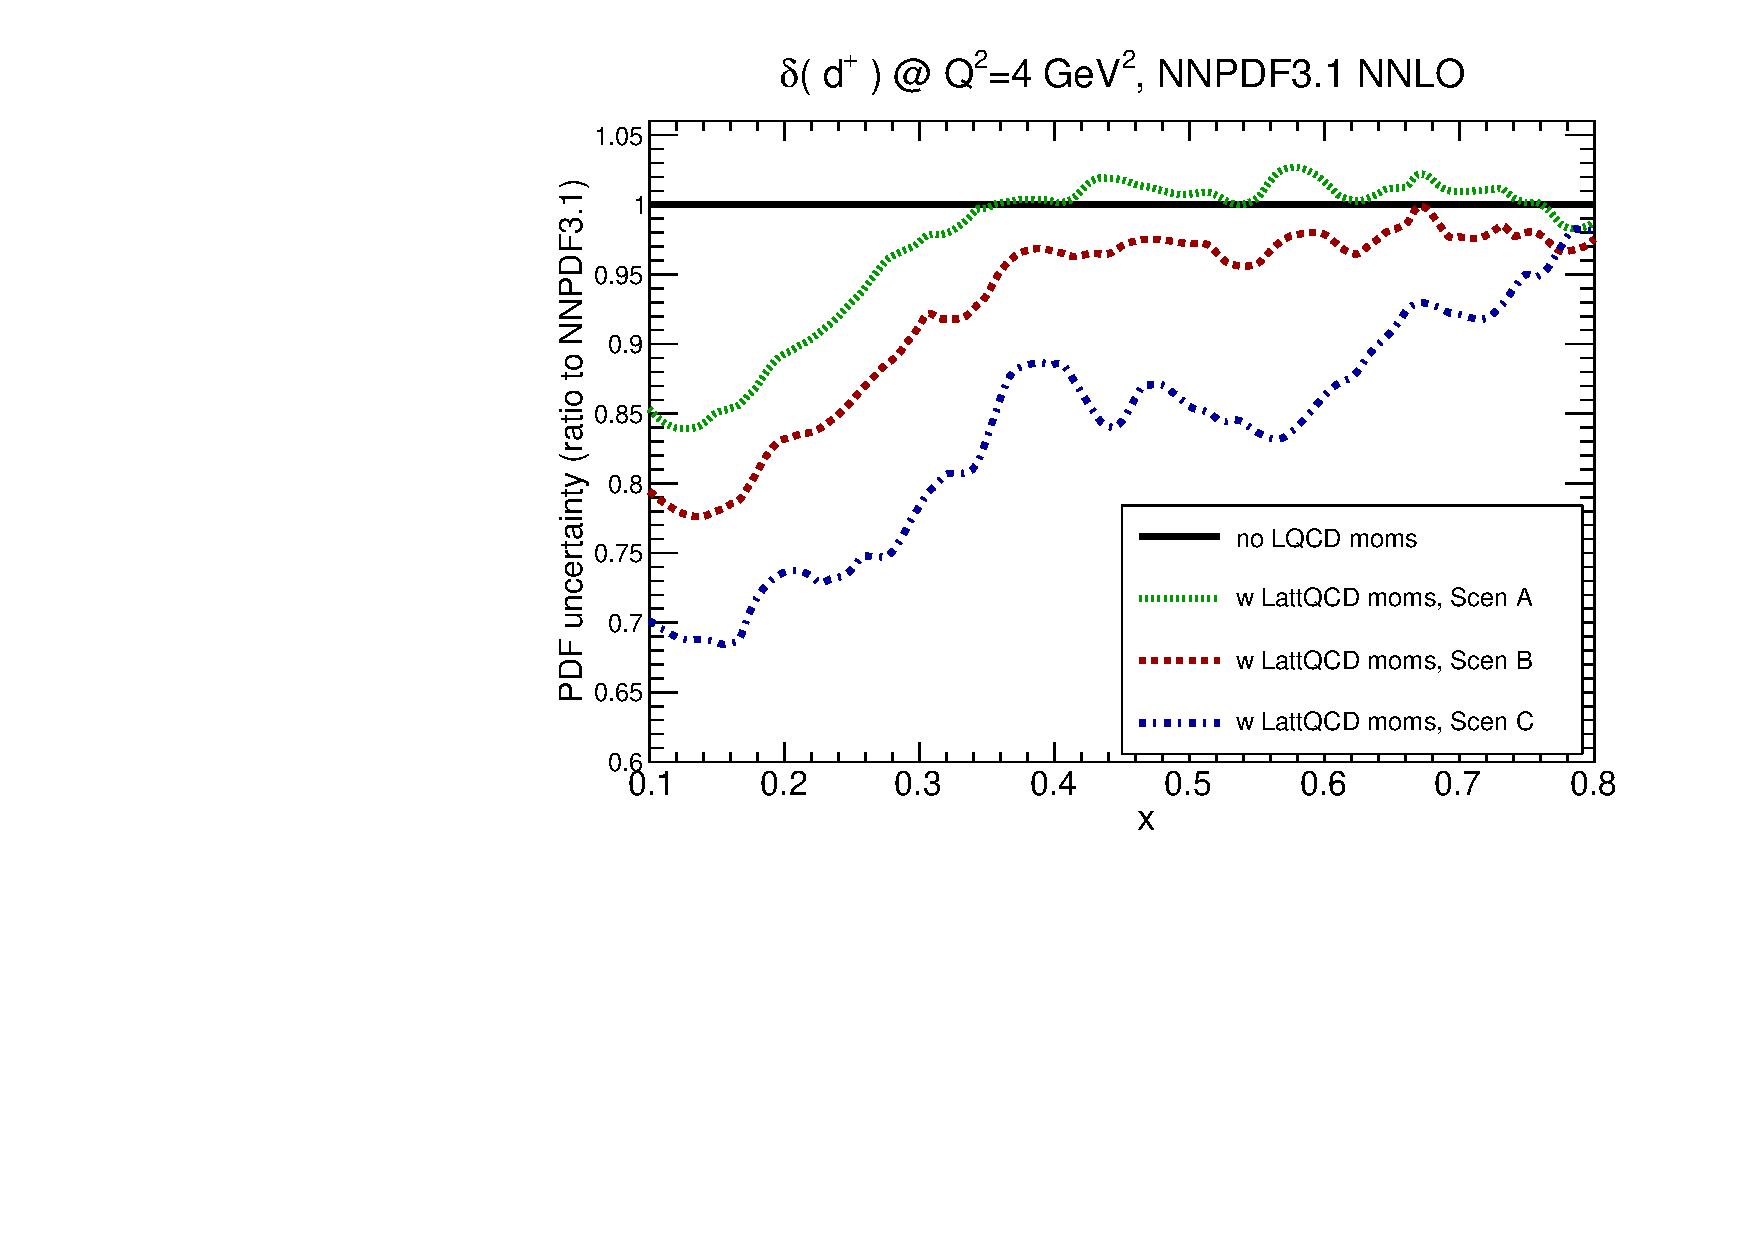
\includegraphics[scale=0.45]{plots/xdp-unpol-lattice-relerr-largex.pdf}
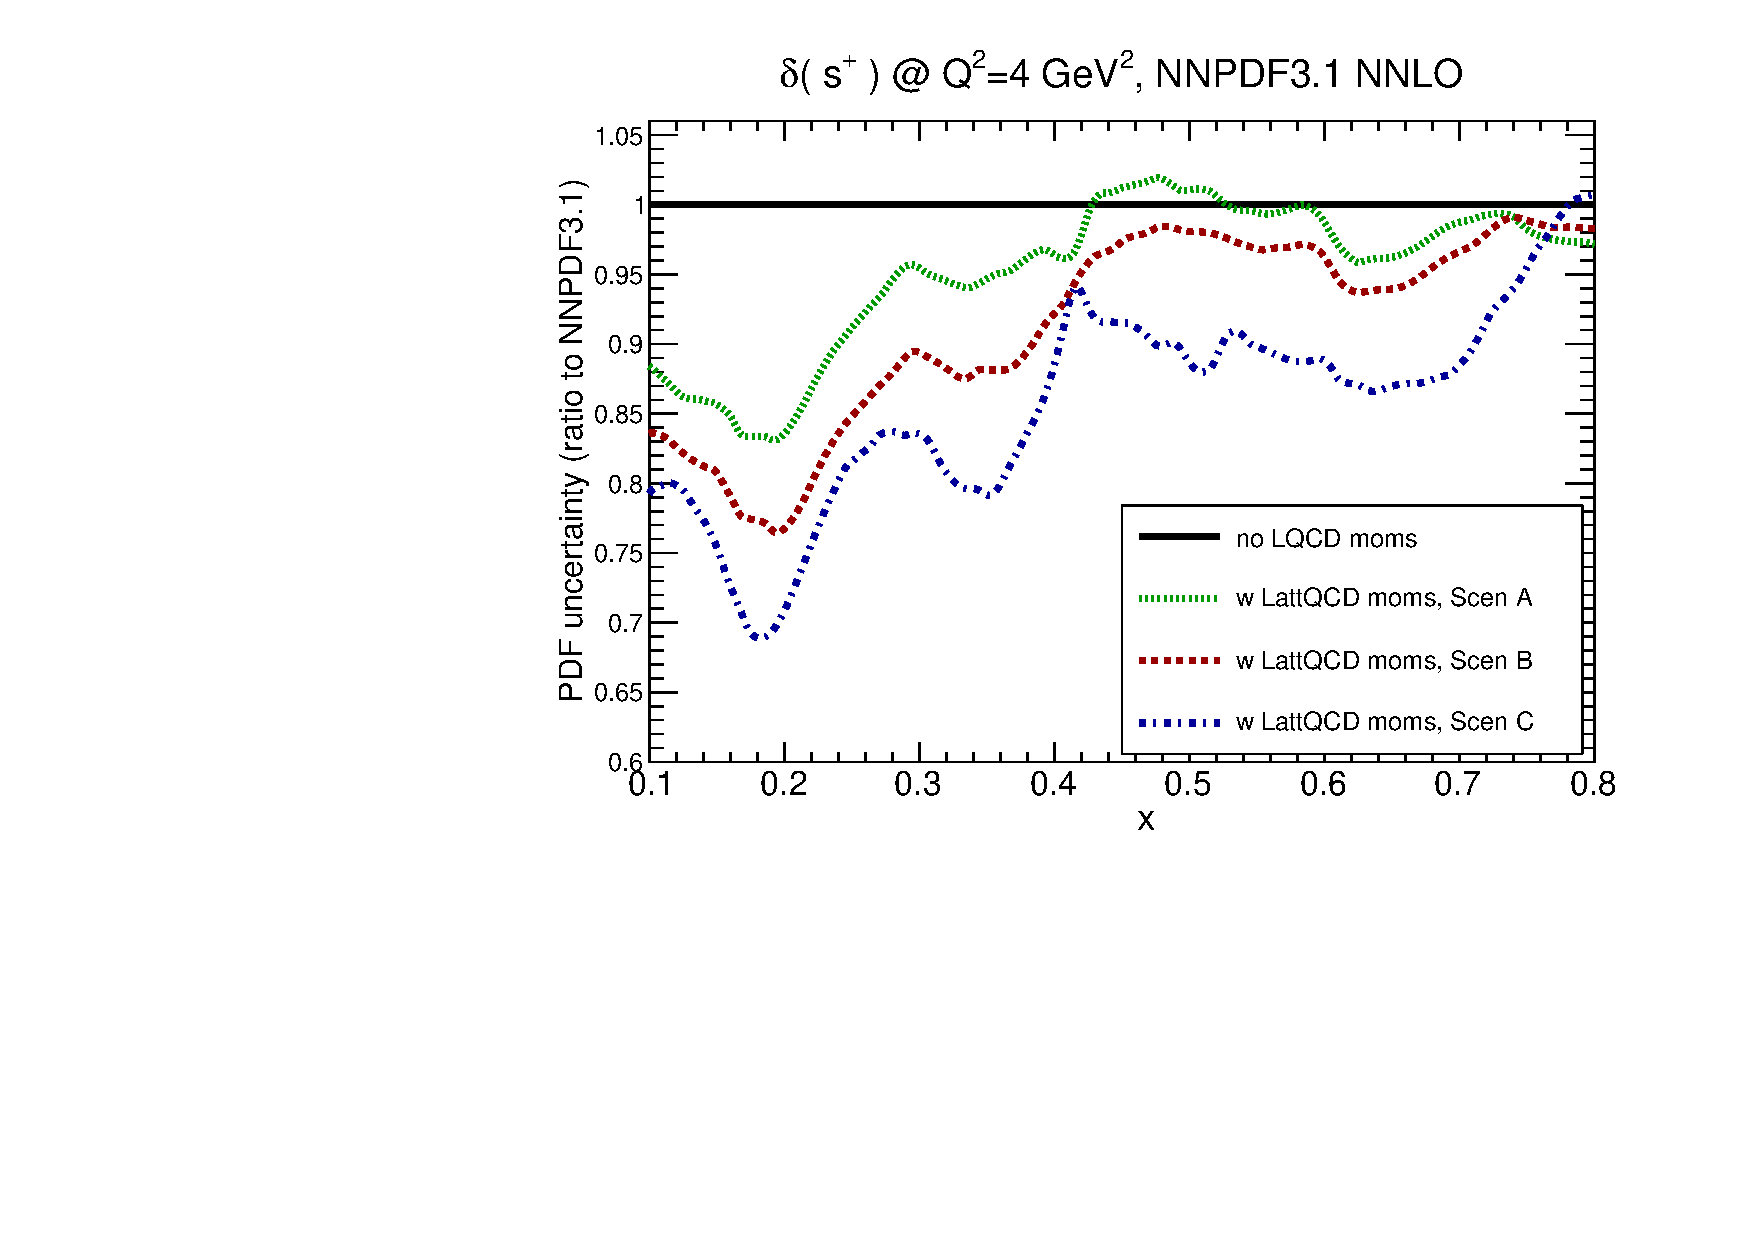
\includegraphics[scale=0.45]{plots/xsp-unpol-lattice-relerr-largex.pdf}
\caption{\small Same as Fig.~\ref{fig:impactUnpol}, now focusing
  on the large-$x$ region, and showing the ratio of the
  PDF uncertainty in the fits based on the three scenarios
  to the original
  PDF uncertainty in the NNPDF3.1 set, for the $d^+$ (left)
  and $s^+$ (right) total quark PDFs.
}    
\label{fig:impactUnpollargex}
\end{figure}
%----------------------------------------------------------

\paragraph{Impact on polarized global fits.}
%
Now we turn to apply the reweighting procedure to NNPDFpol1.1.
%
In Table~\ref{tab:polmomentsrw}
we list the values of the polarized PDF moments
used as pseudo-data, and the corresponding results
after the reweighting has been performed for the
three scenarios summarized in 
in Table~\ref{tab:scenarios}.
%
As in the unpolarized case, the PDF uncertainties quoted correspond in 
all cases to 68\%-CL intervals.
%
As we can see from this comparison, in Scenario~A
(which assumes lattice-QCD pseudo-data with uncertainties similar
to existing calculations) there is a marked impact on the
polarized PDF moments.
%
For both $\la 1\ra_{\Delta u^+}$ and $\la 1\ra_{\Delta d^+}$
the PDF uncertainties are roughly halved, with a similar, but less marked,
trend for $\la 1\ra_{\Delta s^+}$.
%
At this level, there is no impact on the nonsinglet
combinations $\la 1\ra_{\Delta u^+ - \Delta d^+}$
and $\la x\ra_{\Delta u^--\Delta d^-}$.

%-------------------------------------------------------------------------------
\begin{table}[!t]
\centering
\footnotesize
\renewcommand{\arraystretch}{1.4} 
\begin{tabular}{lcccc}
\toprule
& Original & Scenario A &  Scenario B & Scenario C \\
\midrule
$\la 1\ra_{\Delta u^+}$    
& $+0.788 \pm 0.079$   
& $+0.798 \pm 0.039$     
& $+0.797 \pm 0.023$ 
& $+0.790 \pm 0.009$ \\
$\la 1\ra_{\Delta d^+}$   
& $-0.450 \pm 0.083$  
& $-0.450 \pm 0.042$  
& $-0.456 \pm 0.026$    
& $-0.465 \pm 0.012$ \\
$\la 1\ra_{\Delta s^+}$    
& $-0.124 \pm 0.108$  
& $-0.120 \pm 0.070$  
& $-0.121 \pm 0.076$    
& $-0.111 \pm 0.029$ \\
$\la 1\ra_{\Delta u^+ - \Delta d^+}$  
& $+1.250 \pm 0.024$   
& $+1.250 \pm 0.022$  
& $+1.253 \pm 0.016$ 
& $+1.256 \pm 0.012$ \\
$\la x\ra_{\Delta u^--\Delta d^-}$     
& $+0.196 \pm 0.014$    
& $+0.195 \pm 0.014$
& $+0.196 \pm 0.016$     
& $+0.198 \pm 0.012$ \\
\bottomrule
\end{tabular}
\caption{\small Same as Table~\ref{tab:unpolmomentsrw}, now for
  the polarized PDF moments computed with NNPDFpol1.1.
  %
  The corresponding impact at the PDF level is shown in
  Fig.~\ref{fig:impactPol}.
\label{tab:polmomentsrw}
}
\end{table}
%-------------------------------------------------------------------------------

As we further decrease the assumed uncertainties in the lattice-QCD
pseudo-data, we observe a corresponding reduction of the uncertainties
in the global fit.
%
In Scenario~C, the most optimistic, we find that for both
$\la 1\ra_{\Delta u^+}$ and $\la 1\ra_{\Delta d^+}$ there is an uncertainty
reduction by about an order of magnitude compared to the current values,
and by about a factor of five for $\la 1\ra_{\Delta s^+}$.
%
Therefore, future lattice-QCD calculations of
polarized PDF moments can potentially lead to a much more
precise understanding of the spin structure of the proton.
%
The other quark combinations exhibit less sensitivity to the inclusion
of the PDF moments in the global fit, because
they are already quite well constrained by available experimental
data.
%
The PDF uncertainties for  $\la 1\ra_{\Delta u^+ - \Delta d^+}$
are reduced by a factor of two in this quite optimistic scenario, while
those of $\la x\ra_{\Delta u^--\Delta d^-}$ are essentially unaffected even
in the most optimistic scenario.

In Fig.~\ref{fig:impactPol} we compare the absolute PDF uncertainties
of the NNPDFpol1.1 fit to the corresponding results once the lattice 
pseudo-data on polarized moments are included in the analysis by means of the
reweighting.
%
We show absolute rather than relative uncertainties
because, unlike unpolarized PDFs, polarized PDFs often exhibit nodes
(in particular for strangeness and the gluon) and in the nearby regions
the concept of relative uncertainty becomes ill-defined.
  
%-------------------------------------------------------------------
\begin{figure}[!t]
\centering
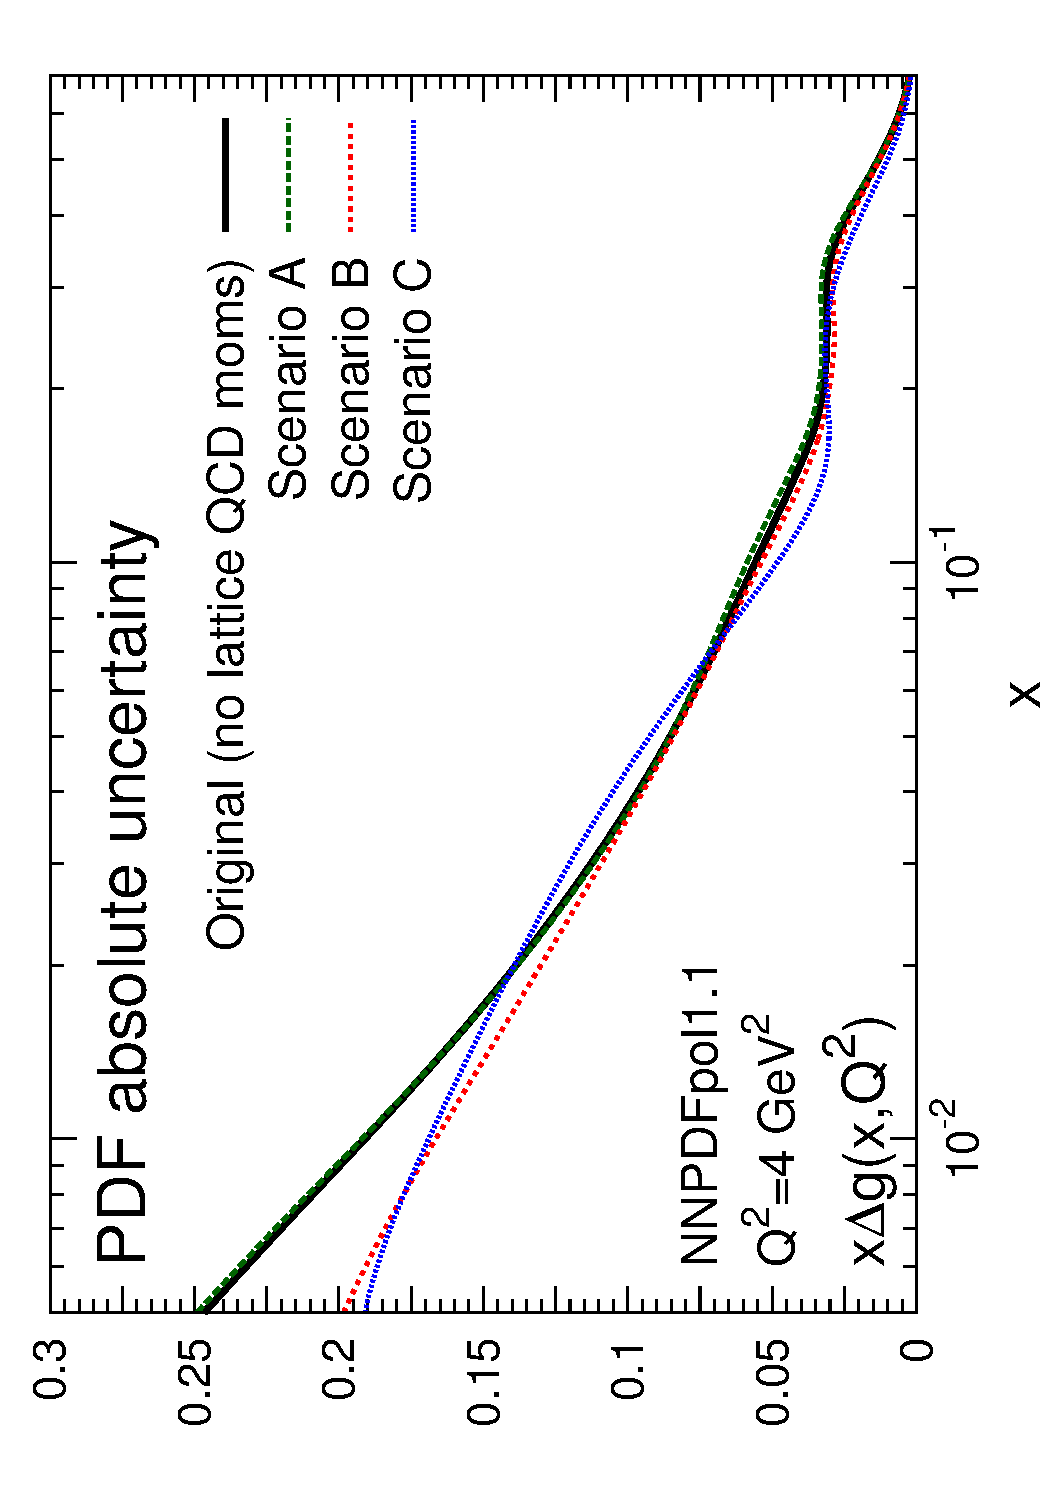
\includegraphics[angle=270,scale=0.35]{plots/POLg}
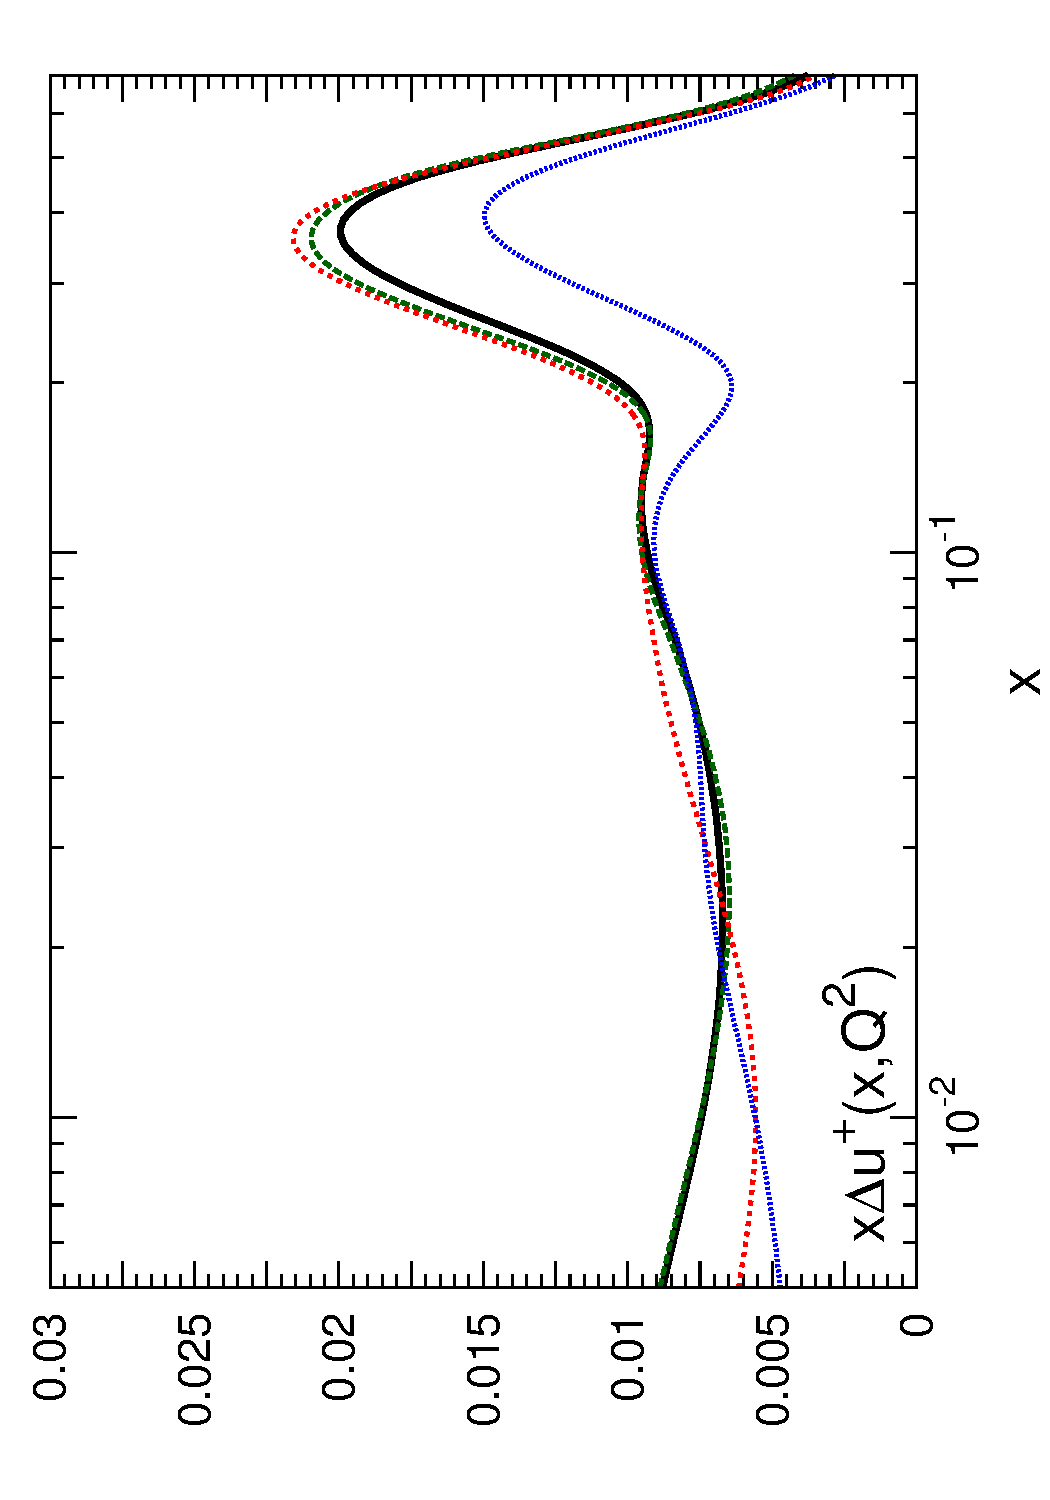
\includegraphics[angle=270,scale=0.35]{plots/POLu}
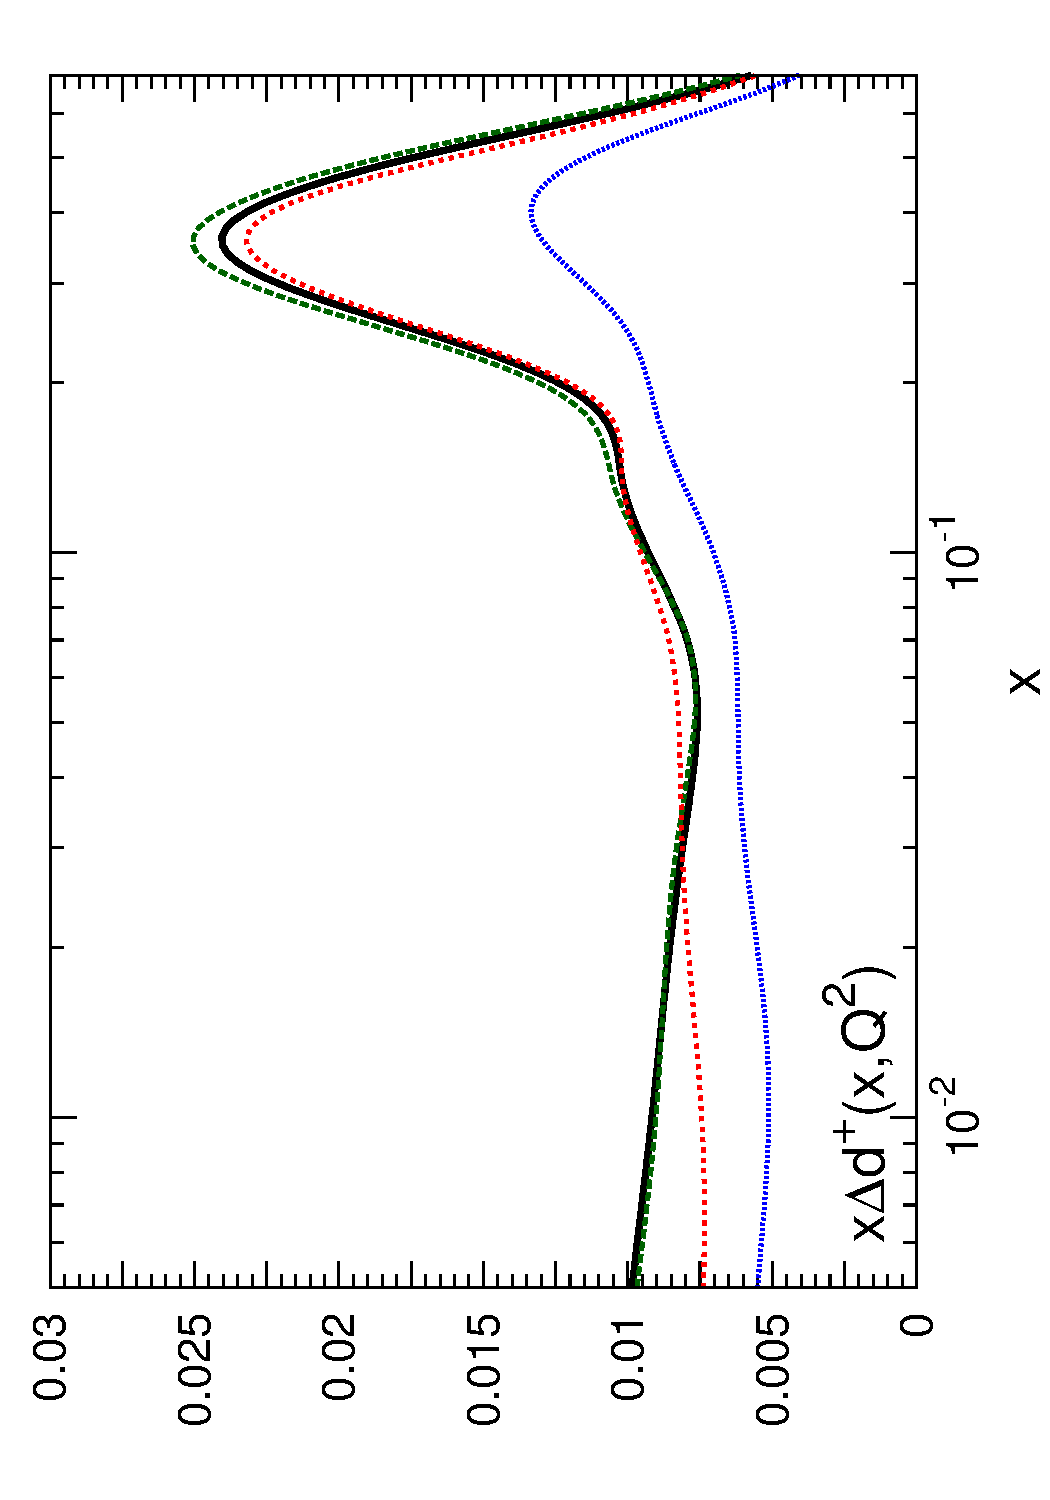
\includegraphics[angle=270,scale=0.35]{plots/POLd}
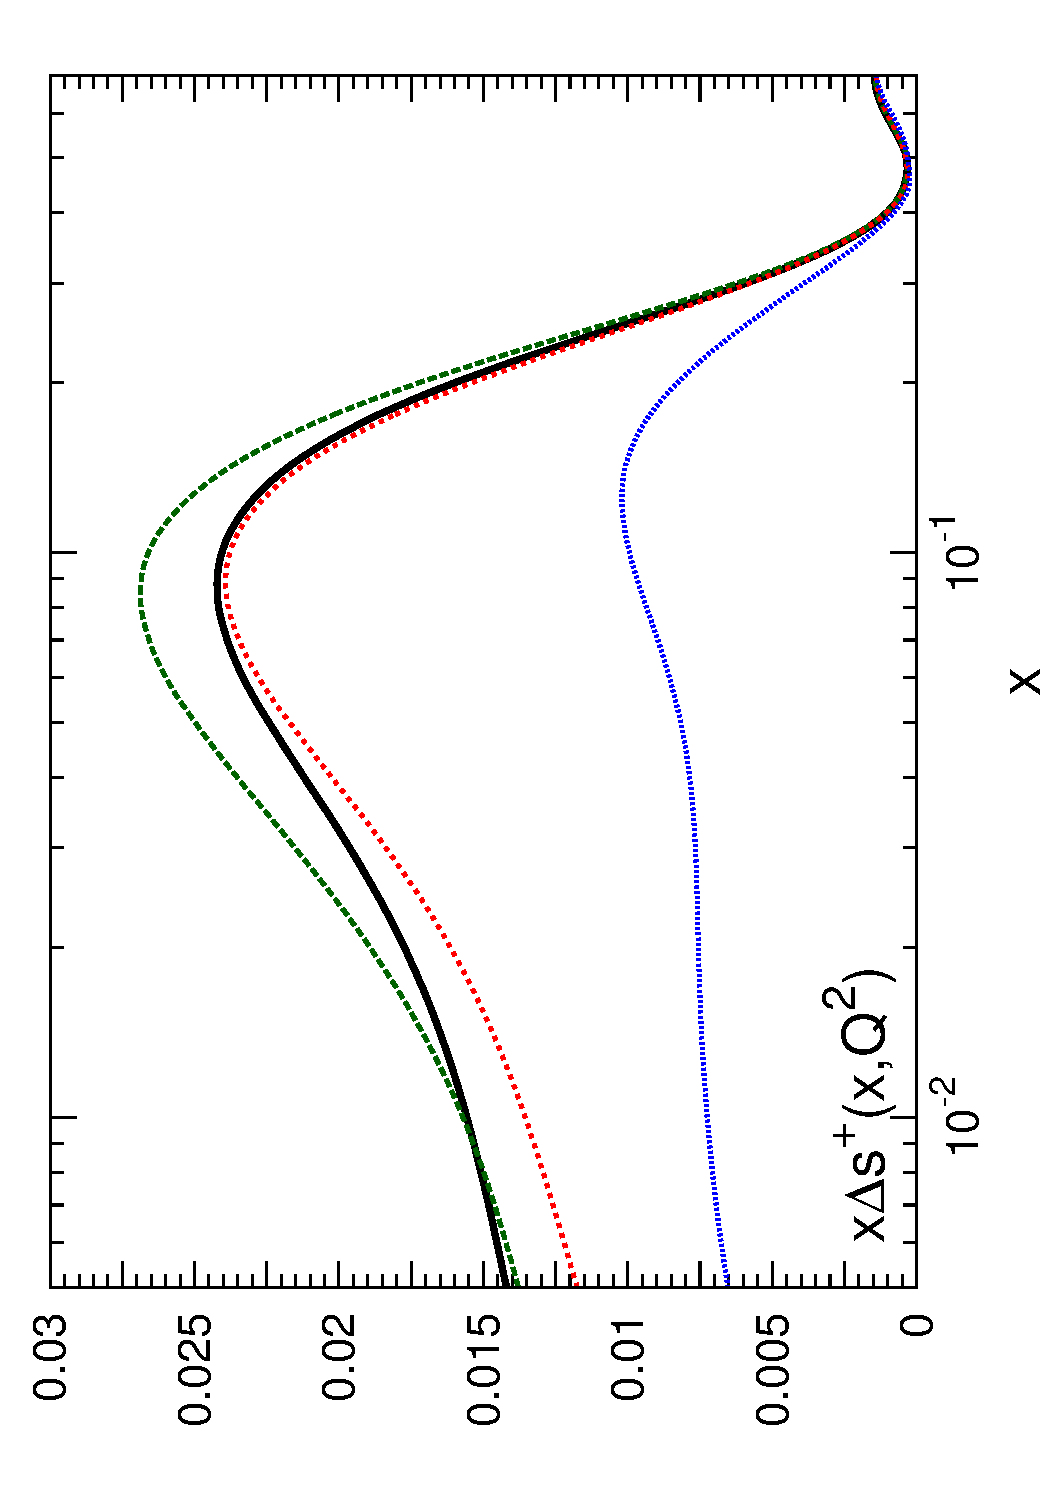
\includegraphics[angle=270,scale=0.35]{plots/POLs}
\caption{\small Same as Fig.~\ref{fig:impactUnpol}, now
  showing the absolute PDF uncertainties of the NNPDFpol1.1 fit
  $Q^2=4\text{ GeV}^2$, compared to the corresponding results once the lattice 
  pseudo-data on polarized moments is included in the analysis via reweighting.
}    
\label{fig:impactPol}
\end{figure}
%---------------------------------------------------------------------

From Fig.~\ref{fig:impactPol} we see that for scenarios
A and B there is only a very moderate reduction (or even a slight increase)
of the PDF uncertainties, seemingly at odds with the results
for their moments in Table~\ref{tab:polmomentsrw}.
%
The reason is that the first PDF moments alone provide only limited
information on the shape of the PDFs themselves, and therefore in some
cases one finds a larger error reduction on the moments (since these
are the fitted quantities) than on the PDFs themselves (which are
only indirectly constrained).
%
Once, however, the lattice-QCD pseudo-data uncertainties
decrease beyond a certain level, these uncertainties start to influence the 
PDF shape, as we can see from the results of Scenario~C.
%
In that case we find that the PDF uncertainties can decrease by up to a factor
of two (three) for $\Delta d^+(x,Q)$ ($\Delta s^+(x,Q)$).
%
We also see the apparently simple feature that relative reduction of PDF 
uncertainties is more or less constant along the whole range of $x$. 
%
For the strange quark this is perhaps roughly consistent with a simple 
reduction in the normalization uncertainty independent of $x$.
%
However, similarly to the unpolarized case, for the down quark this 
decrease is a much smaller factor than the decrease in the uncertainty 
of the moments, meaning that there must be some anticorrelation between 
PDFs at different $x$ values.  


